% 01_Introduction
\chapter{Introduction}
\noindent Integrator is an application that is able to import processed microarray data from different platforms and perform gene-centric integration of those. It holds many novel analysis methods that allow, e.g., integrated pathway-based visualization, gene set enrichment across multiple platforms or integrated tabular views. Integrator can handle directly the following four platforms:

\begin{enumerate}
\item messenger RNA (mRNA) expression data
\item micro RNA (miRNA) expression data
\item protein and protein modification expression data
\item DNA methylation data
\end{enumerate}

Integrator is a high-level data analysis tool. This means, that no low-level data processing methods (normalization, smoothing, etc.) are included in Integrator. The reader is referred to the R statistical computing language to perform low-level data processing for microarrays. But this also means that Integrator supports data from various microarray manufacturers. To import microarray data, Integrator just needs any gene identifier and some statistics, i.e. fold changes or p-values, for each probe. Therefore, it is also possible to use data from other platforms than the mentioned four. Please see the FAQ for more information on this.


Besides developing powerful analysis methods and visualization tools, we have put a huge amount of work to make Integrator as easy-to-use as possible. Therefore, Integrator already includes many pre-processed datasets and mapping files. This also includes, for example, integrated microRNA targets from different databases for multiple organisms or mapping files to convert different IDs to gene symbols.

The detailed list of features is very long and every feature is described in it's own section in more detail. The following is a list of the main features of Integrator:

\begin{itemize}
  \item Getting started:
  \begin{itemize}
  \item Read processed microarray data from tabular text files
  \item Manually import gene lists
  \item Show microRNA targets for human, rat or mouse, choosing one or multiples of the following databases:
  \begin{itemize}
    \item Experimenttally verified
      \begin{itemize}
      \item miRecords
      \item miRTarBase
      \item TarBase
      \end{itemize}
    \item Predicted
      \begin{itemize}
      \item ElMMo
      \item DIANA � microT
      \item TargetScan
      \end{itemize}
  \end{itemize}
  \item Visualize KEGG Pathways
  \end{itemize}


  \item Single dataset analysis:
  \begin{itemize}
  \item Gene set enrichment analysis:
    \begin{itemize}
    \item KEGG Pathway enrichment
    \item Gene Ontology (GO) enrichment
    \item Enrichments using any gene set from the Molecular Signatures Database (MSigDB)
    \end{itemize}
  \item Annotate targets of miRNAs
  \item Pathway-based visualization of any microarray data
  \item Locus-based visualization of DNA methylation data
  \item \dots
  \end{itemize}

  \item Integrated, cross-platform analysis methods (using data from heterogeneous platforms):
  \begin{itemize}
    \item Data pairing (e.g., showing miRNA data together with mRNA targets)
    \item Gene-centered and expandable integrated tabular view of multiple platforms
    \item Integrated gene set enrichment analyis (enrichment across multiple platforms, same databases supported as mentioned before)
    \item Pathway based visualization of microarray data from four different platforms in one pathway
  \end{itemize}


  \item Pathway visualization features:
  \begin{itemize}
    \item Visualization of various KEGG pathways
    \item Highlighting enriched genes from a pathway enrichment analysis directly in a visualized KEGG pathway
    \item Searching/Highlighting of genes/compounds, etc.
    \item Visualization of data directly in a pathway:
    \begin{itemize}
      \item Coloring pathway nodes accorings to an observation (e.g., mRNA fold change)
      \item Adding miRNA nodes with relevant targets to the pathway
      \item Coloring miRNA nodes
      \item Extending pathway-nodes to visualize expression data for various protein modifications
      \item Extending pathway-nodes to show the amount of differential methylation in gene promoters
      \item Showing corresponding observations/ expression values directly in the ToolTip of pathway nodes
    \end{itemize}
    \item Inspecting locus-based DNA methylation regions for specific pathway genes
  \end{itemize}


  \item Application features:
  \begin{itemize}
    \item Easy-to-use and user-friendly
    \item All features are included in one graphical user interface
    \item Automatic detection of file formats and content
    \item Customization of various options via preferences
    \item Help available directly in the application
    \item Cross-linked pathway view (double-click nodes to get more info)
    \item Save and export everything (to multiple formats)
    \item Everything included (targets, mappings,...) and non-included data is downloaded automatically
    \item Multiple FDR correction methods included
    \item Application is available for download and also runs as Java WebStart
  \end{itemize}
\end{itemize}


%%%%%%%%%%%%%%%%%%%%%%%%%%%%%%%%%%
% 02_Installation
%%%%%%%%%%%%%%%%%%%%%%%%%%%%%%%%%%
\chapter{Installation}
Integrator comes as a Java JAR file. It can run out-of-the-box on all systems where a Java virtual machine is installed and does not require any further installations.

\section{Requirements}
\subsection{Software}
Integrator is entirely written in Java\TTra and runs on any operating system where a suitable Java Virtual Machine (JDK version 1.6 or newer) is installed. See, for example, the Java SE download page\footnote{\url{http://www.oracle.com/technetwork/java/javase/downloads/index.html}
\label{fn:jvmldl}}.

\subsection{Hardware}
With at least 1\,GB main memory, you should be able to perform most tasks without any problem.
For large datasets, you should have at least 2\,GB of main memory. \newline
An active internet connection is required for most operations.

\section{Starting the application}
\label{startingTheProgram}
If you downloaded a ZIP-file, you need to unzip it before starting the application. Depending on your operating system, you should use the provided shell scripts for starting the application. This is \texttt{start.sh} for Linux or \texttt{start.bat} for Windows. On MAC OS, you have to create your own shortcut. You can start the application on all operating systems by typing

\begin{lstlisting}[language=bash,numbers=none]
java -jar -Xms128m -Xmx1024m Integrator.jar
\end{lstlisting}

\noindent on your command prompt. In this example, a minimum of 128\,MB and a maximum of 1024\,MB of memory will be available for the program. In most cases, Integrator needs more than 128\,MB memory, so it might be convenient to create a shortcut and start the application with as much memory as available. If you have 2\,GB RAM, for example, you might want to start the application with the following command:

\begin{lstlisting}[language=bash,numbers=none]
java -Xms128m -Xmx1400M -jar Integrator.jar
\end{lstlisting}

For your convenience, we already created several start-scripts to run the application with as much memory as possible. How much memory you actually need strongly depends on the size of your input datasets.
%
\newline\newline \textbf{It is strongly recommended to start the program with at least 1\,GB memory (\texttt{-Xmx1G}).}\newline


\chapter{How to get started}

\section{1. Prepare microarray data}
\label{ch:prepare}

First of all, make sure that your microarray data is in one of the required formats. The application can read character separated value (CSV) files, which are mostly tab-separated tabular files with microarray data. To use EXCEL-data, you can simply open your EXCEL spreadsheet, click "File" and "Save as" and select "Tab-separated text file".
For nearly all data formats, the most important columns are your observations, which can be p-values or fold-changes, and one column with any gene identifier. Supported gene identifiers are gene symbols, NCBI entrez gene ID, Ensembl gene ID, RefSeq ID or KEGG ID.

\emph{Note: Integrator can not process raw data. Please use only processed microarray data.}

\subsection{mRNA expression data}
As always, your file must be formatted as character (preferably tab) separated text file. Necessary columns are only one for the gene identifier and at least one column for your fold-changes or p-values.

Example:
\begin{lstlisting}[caption={Input file example for messenger RNA expression data},label={lst:input:mrna},numbers=none,captionpos=t,float=h]
Gene.Symbol	EntrezGene.ID	Ctnnb1_foldchange	Ras_foldchange
Copg        54161         0.17              0.64
Atp6v0d1    11972         0.04              -0.24
...         ...           ...               ...
\end{lstlisting}



\subsection{miRNA expression data}

MicroRNA datasets are required to be character separated text files. Besides columns with fold-changes or p-values, just one column, containing a systematic miRNA identifier, is required. The systematic name can refer to either the mature, or the pre-miRNA.


Example:
\begin{lstlisting}[caption={Input file example for micro RNA expression data},label={lst:input:mirna},numbers=none,captionpos=t,float=h]
Systematic_name Ctnnb1_foldchange Ras_foldchange
mmu-miR-96      1.45              7.21
mmu-let-7e      -0.72             0.46
...             ...               ...
\end{lstlisting}


\subsection{DNA methylation data}
Integrator can read any DNA methylation data with references to chromosomal locations. This can lead to huge datasets with up to single base pair resolution. To avoid having too much data, it is strongly recommended to summarize the data to bins of, e.g., $50bps$. Most microarray based DNA methylation datasets are already in a perfect format, because the probe length is mostly $50-75bps$.

All probes must somehow be mapped to genes. Therefore, in addition to the fold-change/p-value columns, at least one of the following three columns are required:
\begin{enumerate}
  \item An "Identifier" column that contains a direct (custom) mapping from every probe to a gene
  \item One "Chromosome" column and a "Probe position" column
  \item One column, containing chromosome and position as probe identifier (format: "CHR{chromosome}FS{position}", e.g. "CHR12FS1234"). This is also used by some companies (e.g. Nimblegen) as probe identifier.
\end{enumerate}

In the later two cases, a dialog will appear that let's you choose how to map the data to the genome. Probes can either be mapped to gene bodies or promoter regions. In the later case, you can specify the region up-/ and downstream of a TSS.

\noindent\textbf{Note: it is always recommended to have chromosome and position information with your DNA methylation data. Without these information, creating genome-based plots is not possible!}

Example:
\begin{lstlisting}[caption={Input file example for DNA methylation data},label={lst:input:dnam},numbers=none,captionpos=t,float=h]
Gene               probe_start probe_end ProbeID          Ctnnb1_foldchange
ENSMUSG00000056912 100054458   100054515 CHR10FS100054458 0.08
ENSMUSG00000056912 100053768   100053817 CHR10FS100053768 0.04
ENSMUSG00000046567 100052169   100052221 CHR10FS100052169 0.08
...                ...         ...       ...              ...
\end{lstlisting}


\subsection{Protein modification expression data}

Protein expression datasets, as all other datasets, require a gene-identifier and columns with fold-changes or p-values. Furthermore, it is strongly recommended having a column, indicating the modification of the current protein (phosphorylation, cleavage, acetylation, methylation, etc). This is customized for, e.g. phosphoprotein datasets.

Example:
\begin{lstlisting}[caption={Input file example for protein modification expression data},label={lst:input:protein},numbers=none,captionpos=t,float=h]
Analyte_ID  Gene_Symbol Modification EntrezGene Ctnnb1_foldchange
AKT1        AKT1        basic        11651      0.24
AKT1_P-S473 AKT1        P-S473       11651      -0.34
PRKAA1      PRKAA1      basic        105787     0.07
...         ...         ...          ...        ...
\end{lstlisting}

The modification column indicates, if and how the protein is modified and at which site. For example, "P-S473" indicates a phosphorylation of the serine 473 site. The term "basic" refers to the unmodified protein. These modifications prevent InCroMAP from mixing different values of the same protein, but coming from different protein modifications (example input data may come from reverse-phase-protein-arrays, e.g., from Zeptosense). Moreover, for simple protein expression data (without modification expression information), one can simply omit the modification column.

\section{2. Open microarray data in the application}

\begin{figure}[h]
\centerline{\noindent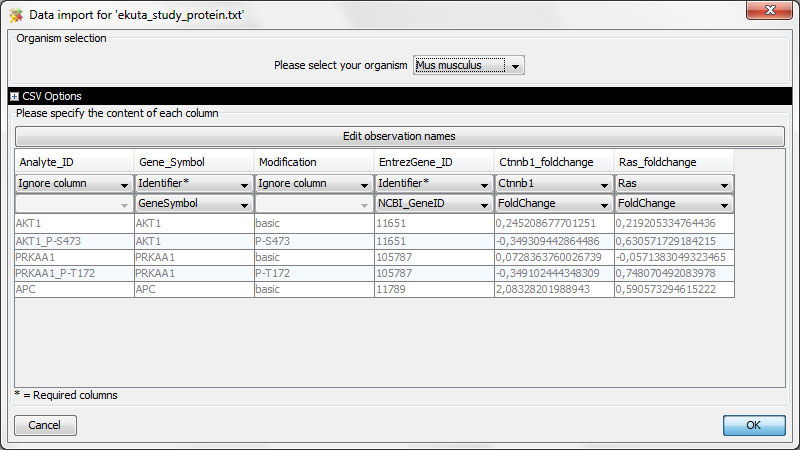
\includegraphics[width=1.0\columnwidth]{figures/import_dialog.jpg}}
\caption{
Example of the data import dialog. On the top, the species must be selected. The "CSV Options" panel might be expanded to correct auto-detected input file properties. At the table in the lower half, the content of each column must be specified.
}\label{fig:inputdialog}
\end{figure}

In general all data must be processed expression data in tabular text files (see Section~\ref{ch:prepare} for descriptions and example of the input file formats). Then, there are many possibilities to open datasets in InCroMAP. For example, you can simply drag\&drop data into the application or select "File", "Open" to open a file. In the upcoming dialogs, you will need to define which type of microarray data is contained (mRNA, miRNA, DNA methylation or protein) and which columns contain what information.

Figure~\ref{fig:inputdialog} shows an example of the file input dialog. First, the species must be selected (on top of the dialog). If the input file format has not been inferred automatically, one may click on the black "CSV Options" label to specify further options (like "column separator char" or if the file contains headers - see Figure~\ref{fig:csvoptions}).


\begin{figure}[h]
\centerline{\noindent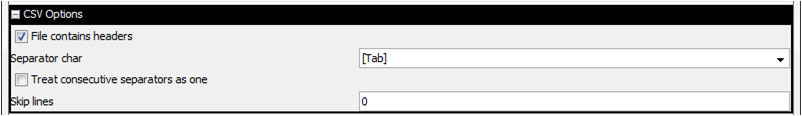
\includegraphics[width=1.0\columnwidth]{figures/expanded_csv_options.jpg}}
\caption{
Expanded "CSV Options" allow to give details for the input file. These properties are auto-detected and only need to be changed if the auto-detection failed to correctly infer those properties.
}\label{fig:csvoptions}
\end{figure}

In the table at the lower half of this dialog, one must specify the content of each column. This can be done by clicking on the combo box below the captions. In some cases (e.g., when selecting "Identifier"), another combo box below the first one will become available and the content must be further specified (e.g., when selecting "Identifier", this can be either a "Entrez Gene ID", "Gene Symbol", "Ensembl Gene ID", etc. - see Figure~\ref{fig:assigngeneid} for an example).

\begin{figure}[p]
\centerline{\noindent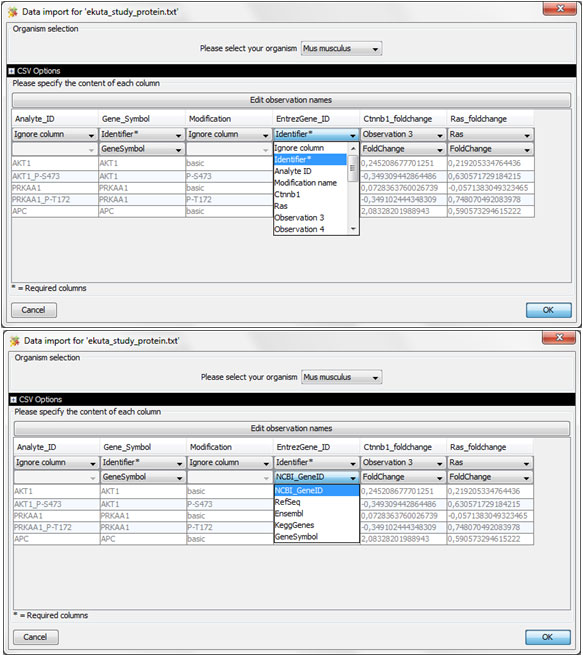
\includegraphics[width=1.0\columnwidth]{figures/assign_geneid.jpg}}
\caption{
Example for specifying column contents. In this example, entrez gene ids are given as the content of one column.
}\label{fig:assigngeneid}
\end{figure}

\subsection{Importing observations from expression data}

Section~\ref{ch:prepare} gives examples for input files and specifies, what columns are required for each data type. Besides the data type specific columns, each dataset must have columns, containing your expression data as processed observations. Currently, these can be fold-changes or p-values. To import the fold-changes or p-values, an observation must be assigned to a column by picking "Observation \{Number\}" from the content combo box. Then, another combo-box will become available, which let's the user choose if the content contains fold-changes or p-values. This step is demonstrated in Figure~\ref{fig:importobservations} and must be performed for all observations one might want to import. The term "Observation" refers to any column content, for which fold-changes or p-values can be calculated.

\begin{figure}[!h]
\centerline{\noindent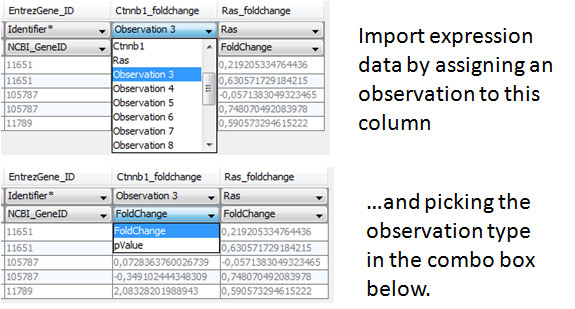
\includegraphics[width=.8\columnwidth]{figures/import_observations.jpg}}
\caption{
Importing processed observations from expression data into the application.
}\label{fig:importobservations}
\end{figure}

\subsection{Renaming observations}

The name "Observation" might be very unspecific for many datasets. Therefore, above the table on the import dialog is a big button "Edit observation names". This button allows renaming all "Observations" to, e.g., "DMSO\_vs\_ko" or more meaningful names. If the input file contained column headers and all observations are already assigned to columns on the input file dialog, InCroMAP will automatically suggest taking the column headers as observations names, as soon as the button "Edit observation names" is pressed. Figure~\ref{fig:renameobservations} demonstrates how to rename observations.

\begin{figure}[h]
\centerline{\noindent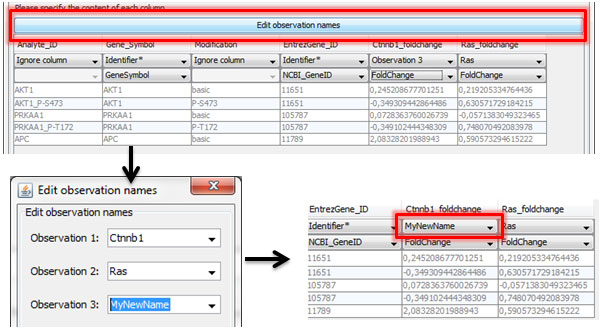
\includegraphics[width=1.0\columnwidth]{figures/renaming_observations.jpg}}
\caption{
To rename observations, click the large "Edit observation names" button. In the upcoming dialog, you may enter new names for each observation. The new name will become effective immediately.
}\label{fig:renameobservations}
\end{figure}

\chapter{Single dataset analysis examples}
This section describes some brief examples how to get started with single dataset analysis in InCroMAP.
As soon as you imported your data into the application, you'll see a table in a new tab, showing your data. On top of the tabs is a toolbar, showing some analysis functions. This toolbar always changes, depending on what is shown in the currently selected tab.

\section{Enrichment analysis (every platform)}
\label{sec:enrichment}
There are two ways of performing an enrichment analysis. On is, to manually select lines in the table (corresponding to probes or genes) and right click on one of the selected lines. Then, you can select an enrichment method (e.g., Gene Ontology or KEGG pathway) to perform this analysis.

The other way is to click the enrichment button in the Toolbar. Then, on needs to select an enrichment type and one will need to define a filter to select probes/genes for an enrichment. For example, in the upcoming dialog one can pick a fold-change column, select "$\mid>=\mid$" (which is the same as "$\geq\pm$") and enter $1.0$ in the last field. This example would lead to an enrichment on all genes that are differentially expressed, with a fold-change cutoff of $1.0$ (i.e. "$fold-change\geq\pm1.0$").

\section{Pathway-based microarray data visualization (every platform)}
There are multiple possibilities to visualize expression data in a pathway-plot, using InCroMAP. On is, for example, to select the tab, containing the table with the input dataset, and click on the "Visualize in pathway" button in the toolbar. In the upcoming dialog, one needs to pick the pathway of interest and an observation, that contains the microarray data that should be visualized in the pathway. This will result in a picture, similar to Figure~\ref{fig:mapkmrna}.

\begin{figure}[htb]
\centerline{\noindent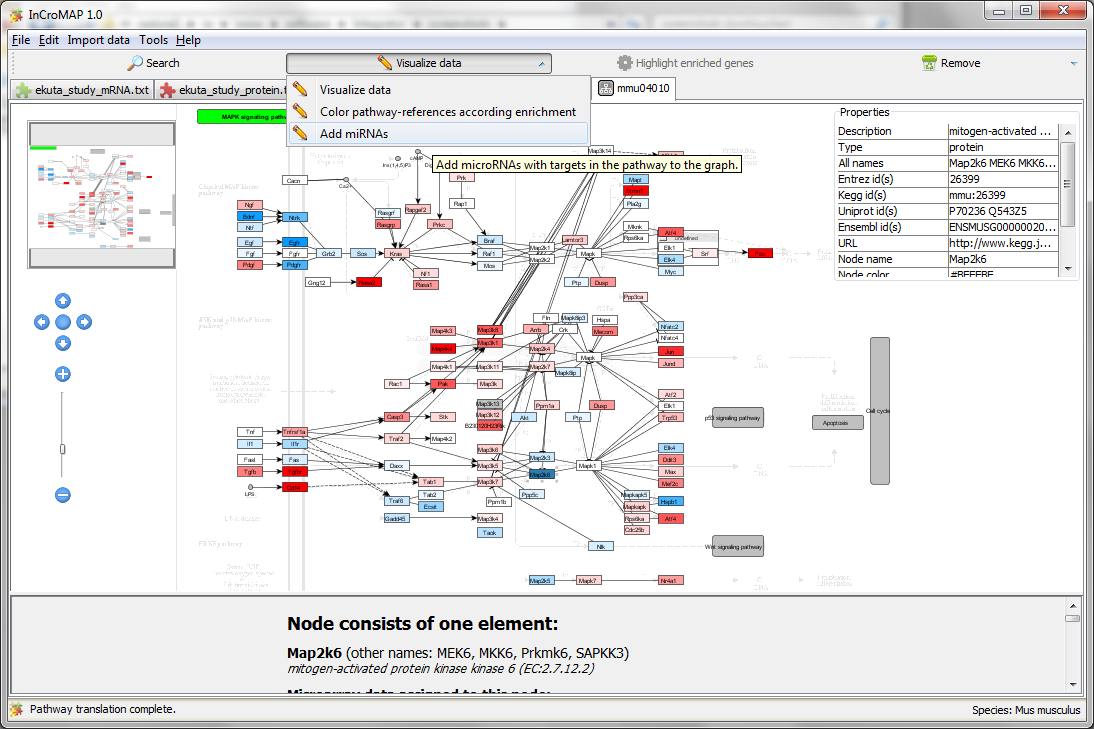
\includegraphics[width=1.0\columnwidth]{figures/9.png}}
\caption{
Example of the "MAPK signaling pathway" with visualized mRNA fold-changes (encoded as node-colors).The "Map2k6" gene-node has been selected and the bottom shows a detail panel, containing detailed information about this gene and all associated expression data.
}\label{fig:mapkmrna}
\end{figure}

Another possibility is to somehow visualize a pathway (e.g., directly from a pathway enrichment analysis or by selecting "Import data" and "Show pathway" from the menu bar) and then click "Visualize data" and again "Visualize data" from the toolbar. See the top of Figure~\ref{fig:mapkmrna} for a screenshot of this option. Then, one needs to select the dataset that should be visualized in the pathway and the observation within this dataset. After clicking "Ok", the data will be visualized in the pathway.

\section{Show microRNA targets (miRNA only)}
\label{sec:showmirnatargets}
When a tab with microRNA data is currently visible, one can select "Targets" and "Annotate targets" from the toolbar. Then, in the upcoming dialog, one can choose which databases should be used to annotate micro RNA targets. There are currently three experimentally derived target databases and three databases with predictions available.

Please note that for all predictions, only targets that are above the suggested "High-confidence" threshold of the cooresponding prediction database have been included in InCroMAP. Targets with low or medium prediction confidence have not been included at all.

Furthermore, many researchers follow the rule that "the more prediction methods suggest a target, the more reliable this information is". This rule has not been implemented into InCroMAP, because this conclusion is wrong. There are multiple reviews, suggesting that it is better to use one good prediction algorithm, than combining multiples with an "OR". The three prediction methods offered by InCroMAP have been proven to be good prediction methods and also to perform good in combination. See \cite{Alexiou2009} for a verification of these statements and further information on micro RNA targets.

\section{Visualize microRNA targets (every platform)}
When a tab, containing a pathway plot (as shown, e.g., in Figure~\ref{fig:mapkmrna}) is currently selected, users can click "Visualize data" and "Add miRNAs" to visualize micro RNAs as small rectangles with edges to their mRNA targets. This can be done, even if no miRNA expression data if available. For more information on the upcoming miRNA target database selection dialog, see Section~\ref{sec:showmirnatargets}.


\section{Genome region plot (DNA methylation only)}

\begin{figure}[htb]
\centerline{\noindent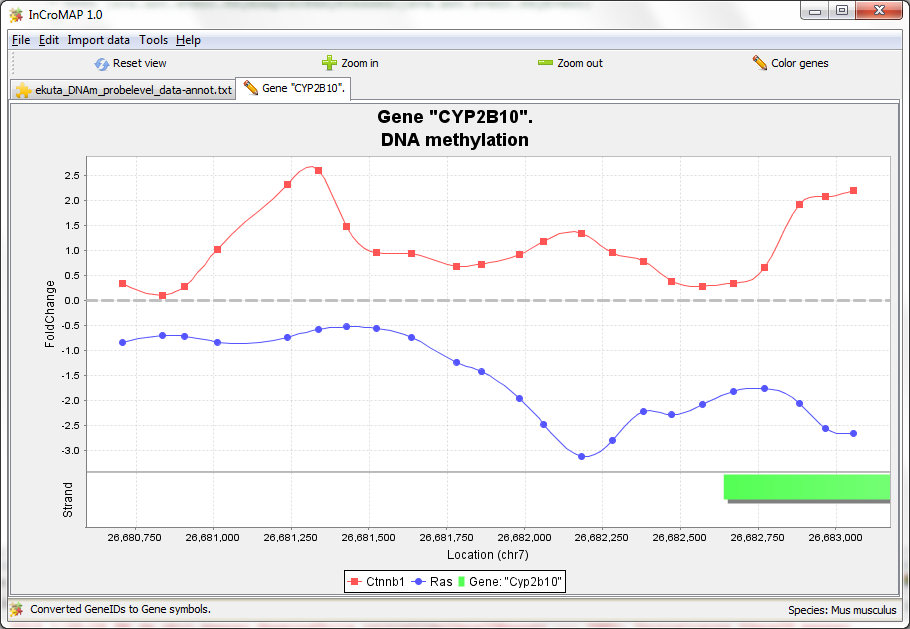
\includegraphics[width=1.0\columnwidth]{figures/me.png}}
\caption{
XY-plot of DNA methylation data in the promoter region of the Cyp2b10 gene.
}\label{fig:dnamplot}
\end{figure}

DNA methylation data can be visualized as genome-region XY-plot. Please select a tab, containing DNA methylation data. There are now two possibilites to generate such a plot: The quick method is by selecting and probe (line in the table), make a right click on it and select "Plot genome region". The application will then collect all probes that are assigned to the selected gene and create a genome plot of them (see Figure~\ref{fig:dnamplot} for an example).

The other possibility is, to click the "Plot genome region" button in the toolbar. The upcoming dialog then let's you pick either a custom region by manually specifying chromosome, start and end coordinates. Or, after clicking "Plot a region, associated to a gene", you can select any gene and let InCroMAP plot all probes that are associated to this gene.
At the bottom of this dialog, you can pick an observation from the current dataset, that should be plotted. To include multiple observations in one plot (e.g., Figure~\ref{fig:dnamplot} has two observations called "Ctnnb1" and "Ras"), one can pick "Include other observations with same signal type" (signal type refers to either p-values or fold-changes). If "Do not include other observations" is selected, only the selected observation will be plotted.


\section{Metabolic overview (mRNA only)}

A good way of getting started with novel mRNA expression datasets is, creating metabolic overviews. This will create a plot, similar to Figure~\ref{fig:metabolicpathways}. As this is an advanced analysis example, please make yourself familiar with the application before trying to follow the described steps.

\begin{figure}[htb]
\centerline{\noindent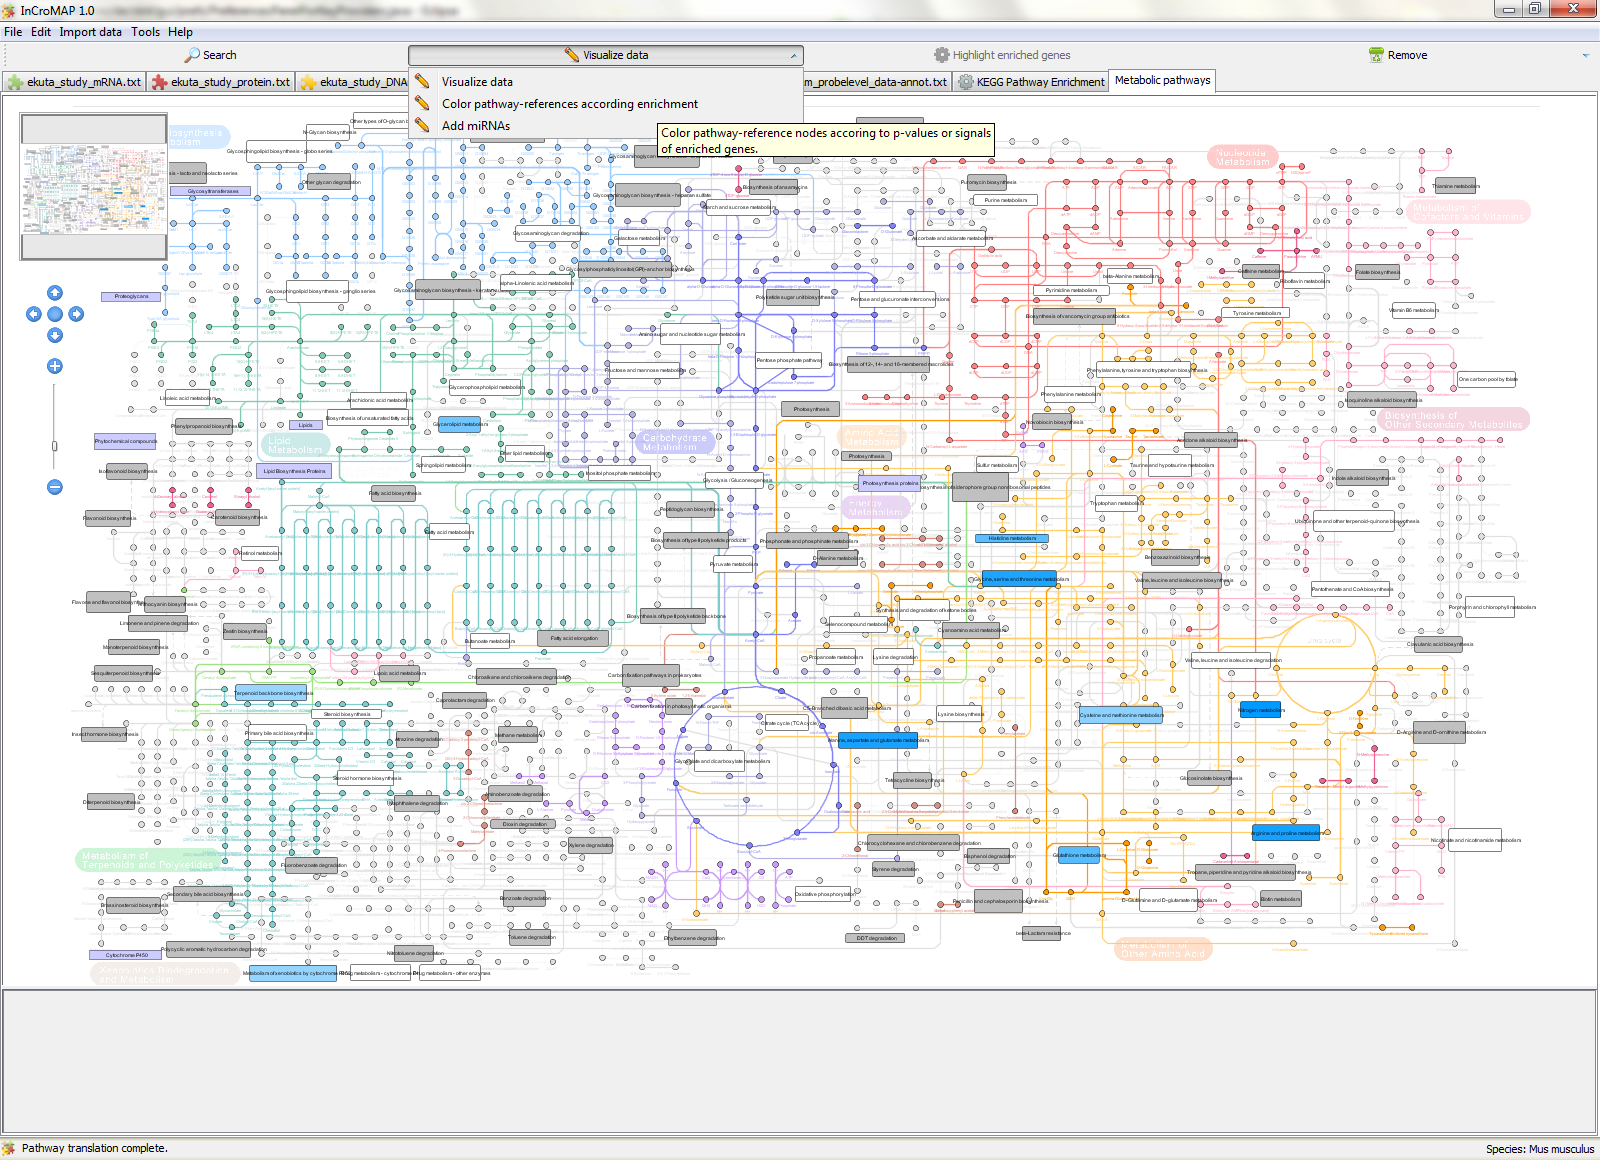
\includegraphics[width=1.0\columnwidth]{figures/mp.png}}
\caption{
InCroMAP visualization of a metabolic overview pathway. All other referenced pathways (rectangle shaped nodes) are colored according to their enrichment p-value (i.e., how significant they are altered in input dataset). The darker-blue they are, the lower the p-value. White means $p-value\geq0.05$ and grey means, that this pathway is not altered at all (not contained in pathway enrichment).
}\label{fig:metabolicpathways}
\end{figure}

From the application, select a tab that contains mRNA data. From this tab, select "Visualize in pathway". In the upcoming dialog pick "Metabolic pathways" from the pathway-selection combo-box and any observation of interest from the combo-box below the pathway selection. After clicking "Ok", the application might need some time to fetch all required data from the KEGG-API.
The result will now be a pathway, similar to Figure~\ref{fig:metabolicpathways}, in which all edges correspond to the mRNA expression level of enzymes. I.e., the colored edges express the mRNA fold-change (or p-value, depending on the selected observation) of the appropriate enzyme. You can click on a colored edge to get more information. Please note that in other pathway, the mRNA expression levels are visualized as colored rectangles, whereas in the "Metabolic pathways"-pathway, all mRNA expression levels are encoded in colored edges!

In this overview-pathway, it is also possible to visualize the importance of specific metabolic pathways. Please go back to your mRNA data tab and perform a KEGG pathway enrichment, as described, e.g., in Section~\ref{sec:enrichment}. Now go back to the metabolic overview pathway again and select "Visualize data" and "Color pathway-references according enrichment" from the toolbar. Select the just performed KEGG pathway enrichment result in the appearing dialog and click "Ok". All nodes, that correspond to references to other pathways (big rectangles with rounded edges) now get colored according to the p-value in the selected pathway enrichment. I.e., the deeper blue they are, the more significant is the enrichment p-value. A white color is assigned to not significantly enriched pathways and grey means, that this pathway is not altered at all (did not appear in the enrichment). Figure~\ref{fig:metabolicpathways} shows an example of the enrichment-based visualization of pathway-reference nodes.


\chapter{Integrated cross-platform microarray data analysis examples}

This chapter describes analysis methods in the InCroMAP application, that are available to users who have data from two or more different platforms for the same samples.

\section{Integrated pathway-based visualization}

TODO: TEXT SCHREIBEN



\section{Data pairing}

\begin{figure}[htbp]
\centerline{\noindent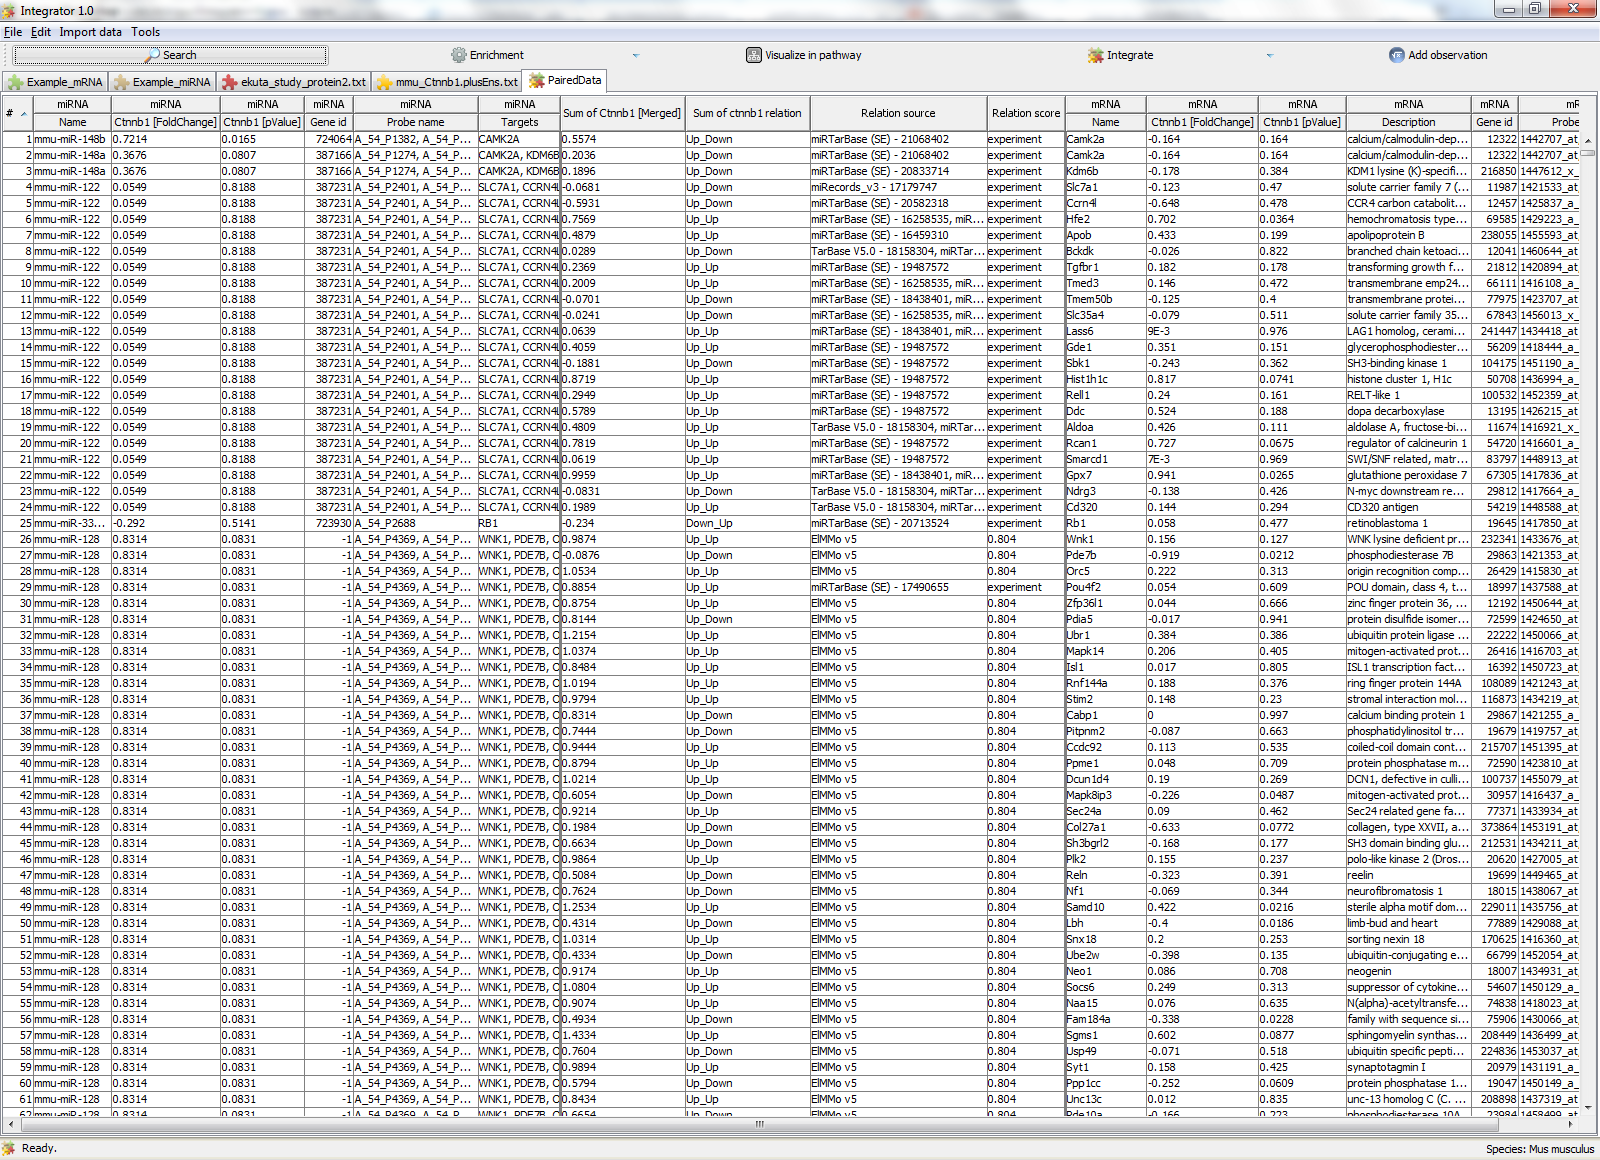
\includegraphics[width=1.0\columnwidth]{figures/e2.png}}
\caption{
Example of the cross-platform "Data pairing" analysis method. Here: an integrated mRNA and microRNA analysis. On the left part of the figure, a micro RNA dataset is shown with expression p-values and fold-changes for each miRNA. In the middle, the target relationship for each miRNA is shown (source database, eventually prediction score, etc.). On the right side, the matching mRNA target is shown together with p-value and fold-change. The "Up\_Down" column in the middle shows the relation of microRNA expression to mRNA expression (i.e., microRNA expression level is upregulated, mRNA expression level is downregulated).
}\label{fig:datapairing}
\end{figure}

Although this method makes especially sense for combinations with miRNA data, it can also be used with any other platform combinations. It basically creates a huge table that puts one dataset in relation to another.
We are going to explain this on some mRNA and miRNA example datasets. The result will be an integrated mRNA and miRNA analysis table, that contains microRNA fold-changes, mRNA target relations, and corresponding mRNA fold-changes (see Figure~\ref{fig:datapairing}). Please select the tab, containing the tabular miRNA data. From the toolbar, select "Integrate" and "Pair data". In the upcoming dialog, you'll need to select the other dataset, which is in our example the mRNA dataset. Furthermore, you have the option to calculate a merged observation. This can be, e.g., the difference between miRNA and targetted mRNA expression fold-change or various other options. You can also unselect "Calculate a merged observation". After pressing "Ok", the paired table with two matched datasets will appear. If you haven't already annotated miRNA data with targets, the target database selection dialog (as described in Section~\ref{sec:showmirnatargets}) will show up before the final results.
The data pairing with micro RNA datasets will lead to three additional columns. One relation column will simplify the miRNA expression fold-change and target fold-change relation. E.g., "Up\_Down" means that microRNA expression is upregulated and the target (e.g., mRNA) expression level is downregulated. The "Relation source" column gives the database(s), that contained or predicted this mRNA to be a target of the miRNA. In case of experimental databases, the PubMed identifier of the corresponding publication is given after the experimental database name. The third additional column is called "Score" and gives the score of the prediction method, if the target is a predicted target. Please refer to the corresponding miRNA target prediction databases itself for an interpretation of these scores. Please note that InCroMAP only shows targets that are above the recommended cutoff threshold for each miRNA target database. I.e. low- or medium confidence targets are not included in InCroMAP at all.

\section{Integrated enrichment}

\section{Gene-based tabular integration of data from multiple platforms}





TODO: Tabellen funktion, auf suche, DNAm plot \& enrichment eingehen und pw visualization einleiten
enrichment, pw visualization separat.
Integrated analysis methods.

- F3 Knopf bei suche
- Tutorial f�r ein downloadbares sample file, von import bis zur enrichment und data in pathway ansicht

2. Open (webstart or download, simply double-click)
3. Analyze

Important Notes (in FAQ?) erkl�rend das kegg merhere gene in 1 knoten zusammenfasst

TODO:
Create a ZIP for download, including start scripts.

TODO PAPER:
Abgrenzung zu GenMAPP und Ingenuity
Application ist auch ein "KEGG Pathway viewer"





TODO: Gliederung:

mRNA data analysis
miRNA data
DNAm
protein

Enrichment Tab

Pathway-tab

Integrated analysis






% 03_Troubleshooting
\chapter{FAQ / Troubleshooting}
Please note: There are separate FAQs for steps 1 (see Section \ref{sec:STEP1FAQ}), 2 (see Section \ref{sec:STEP2FAQ}) and 3 (see Section \ref{sec:STEP3FAQ}).\newline

\noindent \textbf{I'm getting a ``java.lang.OutOfMemoryError: Java heap space"}\newline
Some operations need a lot of memory. If you simply start Integrator, without any JVM parameters, only 64\,MB of memory are available. Please append the argument \texttt{-Xmx1024M} to start the application with 1\,GB of main memory. See Section \ref{startingTheProgram} for a more detailed description of how to start the application with additional memory. If possible, you should give the application 2\,GB or more of memory. Especially reading DNA methylation datasets takes a huge amount of memory.\newline

\noindent \textbf{Is an internet connection required to run Integrator?}\newline
An internet connection is required for most operations. Many identifier mapping files and pathway-based visualization require an active internet connection. However, if you import your data directly with NCBI Entrez Gene IDs and do not use the pathway-visualization or GO-enrichment, you should be able to run the application offline.\newline

\noindent \textbf{Which organisms are supported?}\newline
Currently mouse, human and rat are supported.\newline

\noindent \textbf{Can I import other microarray data types than the mentioned four?}\newline
Yes! Basically, everything than can be mapped to a gene can be imported. It is recommended to pick the mRNA data type (even if you don't have mRNA data), select any gene identifier and import your data as processed p-values or fold changes. With this method, you can perform integrated analysis, enrichment analysis and pathway-based-visualization of basically every microarray type.


\noindent \textbf{Where can I get the latest version?}\newline
Go to \url{http://www.cogsys.cs.uni-tuebingen.de/software/Integrator/}.


TODO: include items from KEGGtranslator FAQ (missing reactions and such).

TODO: Warum keine miRNA annotiert? (o.�,) => Falscher organismus gew�hlt.

TODO: Signal / Observation generell erkl�ren was damit gemeint ist


